\section{Zweidimensionales Gabor-Wavelet}
\rhead{Zweidimensionales Gabor-Wavelet}

Die Idee des eindimensionalen Gabor-Wavelets wird zuerst als Grundlage genommen. 
Daraus wird dann das zweidimensionale Wavelet abgeleitet und die entstehenden Freiheitsgrade erläutert.

\subsection{Gabor-Wavelet}

Bei der Wavelet-Transformation besteht eine Zeit-Frequenz-Unschärfe.
Diese Unschärfe bewirkt, dass die Auflösung im Zeitbereich umgekehrt proportional zur Auflösung im Frequenzbereich ist.
Das Gabor-Wavelet stellt einen optimalen Kompromiss aus Zeit-und Frequenzauflösung dar.
Die Anwendung des Wavelets minimiert dabei das Produkt der Standardabweichungen im Zeit- und Frequenzbereich. \cite{paper:communication}
%TODO more details?

Ein solches Gabor-Wavelet besteht aus einer komplexen Schwingung, welche mit einer Gaussfunktion gefenstert ist und somit exponentiell abfällt.

\begin{equation}
G(x)= e^{-\frac{(x-x_{0})^{2}}{\sigma^{2}}} e^{i\xi_{0}x}
\end{equation}

%TODO insert description of equation

Die komplexe Schwingung besteht aus einem Sinus und einem  Kosinus Anteil. 
Ein solches Sinus-Gabor-Wavelet wird in Abbildung \ref{fig:gabor1d} gezeigt.

\begin{figure}
	\centering
	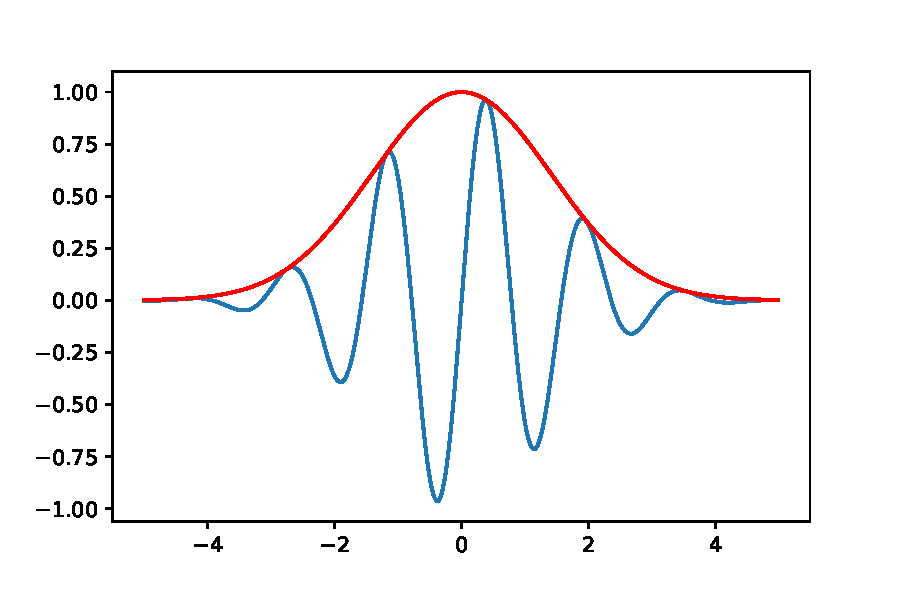
\includegraphics[width=0.7\linewidth]{./papers/visuell/images/gabor_1d}
	\caption{Beispiel eines Sinus-Gabor-Wavelets}
	\label{fig:gabor1d}
\end{figure}


\subsection{Erweiterung auf zwei Dimensionen}

Um ein solches Wavelet auf ein Bild anwenden zu können, ist es sinnvoll dieses auf zwei Dimensionen zu erweitern.
Diese Erweiterung ergibt die folgende Formel:

\begin{equation}
G(x,y)= e^{-(\frac{(x-x_{0})^{2}}{\sigma^{2}}+\frac{(y-y_{0})^{2}}{\beta^{2}})}
e^{i(\xi_{0}x+\nu_{0}y)}.
\end{equation}

Das zweidimensionale Wavelet besteht immer noch aus einer komplexen Schwingung multipliziert mit einer elliptischen Gaussfunktion. 
Diese Schwingung kann man sich als ebene Welle vorstellen, welche abhängig von $\xi$ und $\nu$ in eine bestimmte Richtung zeigt (vgl. Abbildung \ref{fig:planarwave}).

\begin{figure}
	\centering
	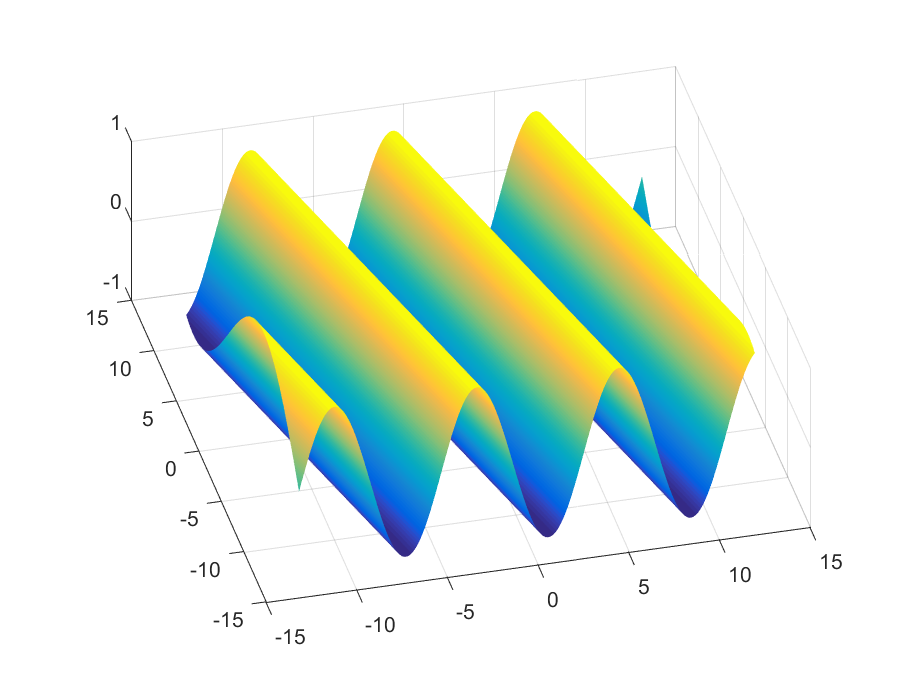
\includegraphics[width=0.7\linewidth]{./papers/visuell/images/planarwave.eps}
	\caption{Beispiel einer ebenen Welle}
	\label{fig:planarwave}
\end{figure}



Diese Parameter ($\sigma$, $\beta$, $\xi$, $\nu$) dieser Formel sind unhandlich und es ist nicht offensichtlich was eine Änderung dieser bewirkt.
Also ersetzen wir diese durch neue Parameter und erhalten 

\begin{equation}
G(x,y)=e^{-\frac{x'^{2}+\gamma^{2}y'^{2}}{2\sigma^{2}}}
e^{i(2\pi\frac{x'}{\lambda} + \phi)},
\end{equation} 
wobei $x'=x\cos(\theta)+y\sin(\theta)$ und $y'=-x\sin(\theta)+y\cos(\theta)$.
Der Parameter $\gamma$ beschreibt das Verhältnis der Streckung in $x$- und $y$-Richtung.
Diese Streckung der Gaussfunktion ermöglicht es ellipsenförmige Wavelets zu erhalten.
Die Standardabweichung der Gausskurve welche mit der Schwingung multipliziert wird ist als Parameter $\sigma$ definiert.
Grösseres $\sigma$ bewirkt ein breiteres Wavelet.
Die komplexe Schwingung wird durch die Wellenlänge $\lambda$ und die Phase $\phi$ definiert.
Der Parameter $\theta$ definiert nun die Ausrichtung der komplexen Schwingung.
Eine Änderung von $\theta$  bewirkt somit eine Drehung der Wellenfronten.

Wie sich Gabor-Wavelets in Abhängigkeit dieser Parameter Verhalten zeigt Abbildung TODO. %TODO insert ref and image
